\section{ViT-B/32 八任务逐任务明细}
\label{apdx:ink-vitb32-details}

表~\ref{tab:ink-vitb32-results} 给出 CLIP ViT-B/32 八任务基准上各方法的逐任务测试准确率，作为正文表~\ref{tab:ink-vision-summary} 中该列平均值的展开。粗体和下划线分别标记所列合并记录中的最优与次优。

\begin{table}[!htbp]
  \centering
  \caption{CLIP ViT-B/32 八任务逐任务明细（\%）。粗体和下划线分别标记所列合并记录中的最优与次优。Individual FT 为独立专家参考。}
  \label{tab:ink-vitb32-results}
  \setlength{\tabcolsep}{2.4pt}
  \renewcommand{\arraystretch}{1.04}
  \resizebox{\textwidth}{!}{%
  \begin{tabular}{@{}lrrrrrrrrr@{}}
    \toprule
    方法 & Cars & DTD & EuroSAT & GTSRB & MNIST & RESISC45 & SVHN & SUN397 & 平均 \\
    \midrule
    Zero-shot & 56.54 & 41.91 & 39.15 & 32.81 & 53.91 & 57.94 & 28.77 & 62.51 & 46.69 \\
    Weight Avg. & 58.86 & 48.35 & 65.78 & 64.94 & 92.42 & 67.97 & 72.80 & 60.21 & 66.42 \\
    Task Arith. & 57.74 & 48.03 & 66.48 & 66.52 & 93.69 & 66.67 & 74.46 & 58.34 & 66.49 \\
    TIES & 59.68 & 50.16 & 65.04 & 70.42 & 97.22 & 70.41 & 82.91 & 59.44 & 69.41 \\
    Consensus TA & 58.99 & 51.44 & 71.04 & 73.56 & 97.37 & 68.75 & 83.19 & 58.52 & 70.36 \\
    Iso-C & 70.00 & 65.37 & 88.33 & 90.74 & 98.82 & 84.68 & 86.72 & 65.95 & 81.33 \\
    Iso-CTS & 69.32 & 65.53 & 88.81 & 91.07 & 98.84 & 84.90 & 84.93 & 64.92 & 81.04 \\
    TSV-M & 68.86 & 64.73 & 91.19 & 90.95 & 99.11 & 81.81 & 89.89 & 64.24 & 81.35 \\
    RegMean & 66.87 & 64.15 & 93.41 & 87.71 & 98.31 & 82.29 & 91.22 & 66.23 & 81.27 \\
    WUDI & 68.23 & 65.90 & 94.11 & 92.45 & \textbf{99.31} & 82.10 & 92.86 & 65.44 & 82.55 \\
    LiNeS (Iso-C) & 72.91 & 69.31 & 92.33 & 92.56 & 99.10 & 86.73 & 86.87 & 67.14 & 83.37 \\
    CoM & 67.14 & 66.65 & \underline{95.26} & 91.70 & 98.93 & 85.17 & \underline{94.76} & 67.41 & 83.38 \\
    ESM & 73.27 & \underline{71.44} & 91.04 & \underline{93.17} & \underline{99.30} & \underline{88.24} & 90.48 & 66.55 & \underline{84.19} \\
    SVC (Iso-CTS) & 72.29 & 67.45 & 88.81 & 89.59 & 98.24 & 85.51 & 81.65 & \underline{69.32} & 81.61 \\
    SVC (ESM) & \textbf{74.00} & 65.96 & 89.74 & 88.72 & 98.92 & 85.02 & 87.62 & 69.09 & 82.38 \\
    \midrule
    \textbf{\method{}} & \underline{73.91} & \textbf{71.76} & \textbf{97.44} & \textbf{96.27} & 99.23 & \textbf{90.03} & \textbf{95.91} & \textbf{71.01} & \textbf{86.95} \\
    \midrule
    Individual FT（上界） & 76.30 & 77.71 & 99.89 & 99.10 & 99.70 & 95.48 & 97.51 & 73.79 & 89.93 \\
    \bottomrule
  \end{tabular}%
  }
\end{table}


在所列合并记录中，\method{} 在 DTD、EuroSAT、GTSRB、RESISC45、SVHN 和 SUN397 的数值最高，Cars 次高，MNIST 低于 WUDI 和 ESM。

\FloatBarrier
\section{单轮更新步长诊断（待验证）}
\label{apdx:ink-step-size}

本节将准确率与 KL 拆为两个独立小节和图，说明为什么几何目标的候选解未必适合直接完整替换当前权重。\textbf{以下曲线仅为可能趋势，不是实测结果}，两图的纵轴均无数值刻度。

\paragraph{先固定同一个候选方向。}
对每个预先固定的校准种子，只从初始化模型估计一次第一轮几何、求解一次候选权重 $W^\star$，然后构造
\[
  W(\omega)=W^{(0)}+\omega\bigl(W^\star-W^{(0)}\bigr),\qquad
  \omega\in\{0,0.1,\ldots,1.0\}.
\]
每个 $\omega$ 都从同一 $W^{(0)}$ 插值，不能在上一个步长的模型上累计更新。扫描期间不重新估计几何、不执行逐块精调；非合并参数保持初始化值。$\omega=0$ 是当前 Iso-C 初始化而非 Zero-shot，$\omega=1$ 才是完整采用第一轮候选解。

\subsection{步长对准确率的影响}
\paragraph{要做什么。}
对上述 11 个模型，在预先固定的测试协议下计算八任务等权平均准确率。未来对每个种子记录原留出 KL 在原候选集合中选出的全局步长，分别标注而不把多个种子的位置平均成一个实际步长。若该步长不在 0.1 间隔网格内，可额外评价其模型，但不得据测试结果重新选步。

\begin{figure}[!htbp]
  \centering
  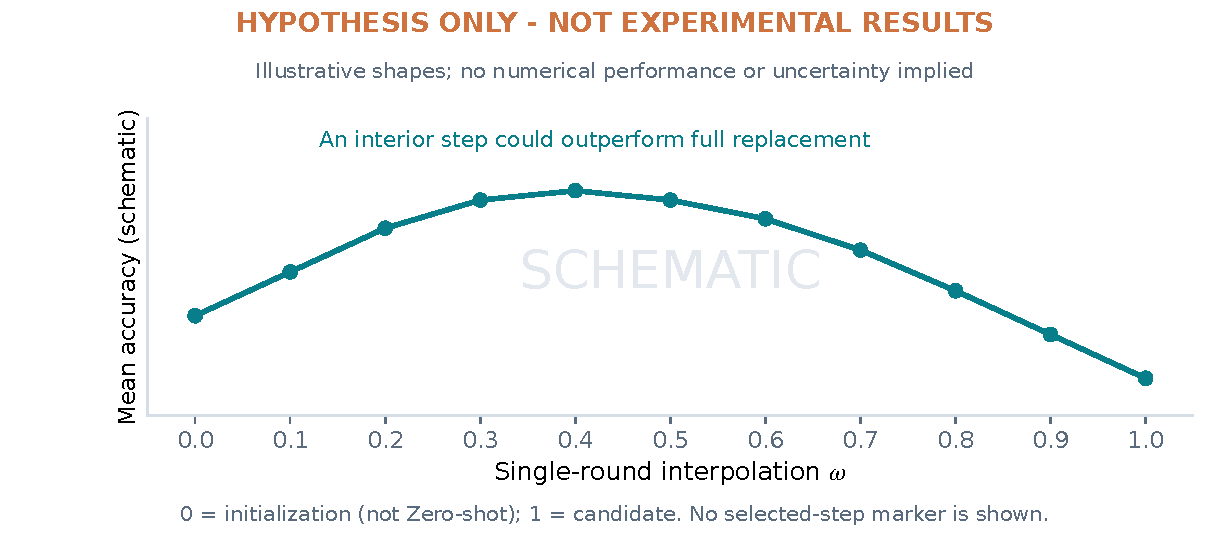
\includegraphics[width=0.78\linewidth]{figures/hypothesis_step_accuracy.pdf}
  \caption{\textbf{单轮步长--准确率的预期趋势示意，非实验结果。}可能的情形是中间步长优于完整替换；示意峰值不对应推荐步长。$\omega=0$ 为初始化模型而非 Zero-shot，$\omega=1$ 为完整候选更新。图中没有实际选步标记。}
  \label{fig:ink-step-size-analysis}
\end{figure}


\paragraph{如何解读。}
图~\ref{fig:ink-step-size-analysis} 示意一种可能的先升后降关系：适度更新恢复任务功能，而完整替换可能过度改变当前模型。若真实 $\omega=1$ 反而最好，则不能用该轮准确率支持保守更新；若多数步长都差，也需检查候选方向本身。图中的峰值位置完全是画图示意，不代表建议使用 $0.4$，也不是完整多轮、逐块 \method{} 的结果。

\clearpage
\subsection{步长对教师 KL 的影响}
\paragraph{要做什么。}
保持上一小节的模型集合不变，在未参与统计、步长与轮次选择的独立诊断集上计算教师--学生 KL，先按任务平均，再对八个任务等权平均。原留出 KL 选步只是标注对象，不能改由独立诊断集或测试集选择。本图与准确率图分开作图，不使用双纵轴。

\begin{figure}[!htbp]
  \centering
  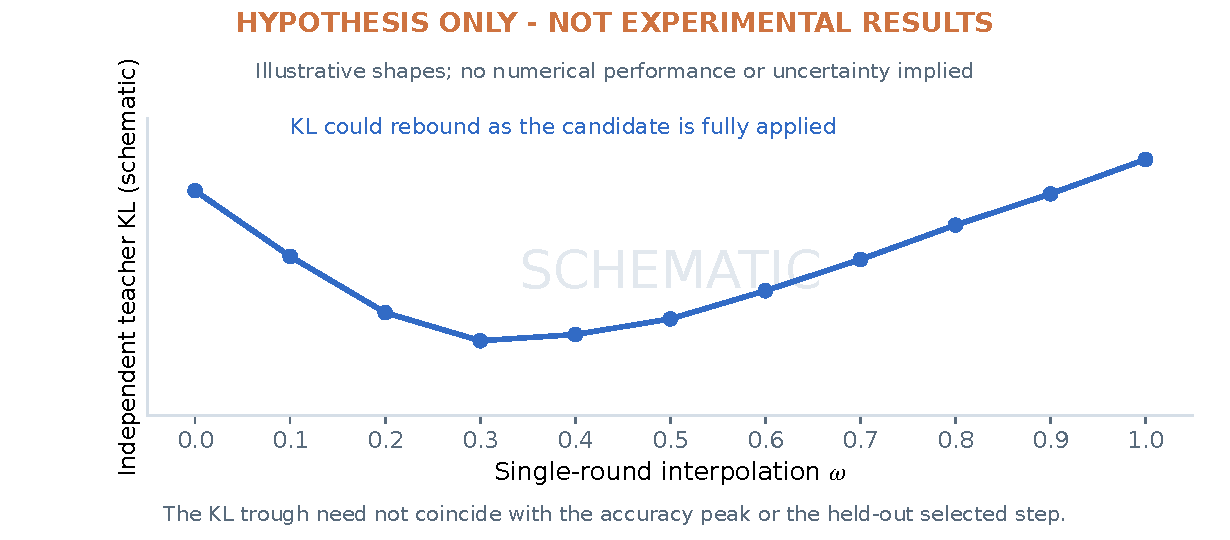
\includegraphics[width=0.78\linewidth]{figures/hypothesis_step_kl.pdf}
  \caption{\textbf{单轮步长--教师 KL 的预期趋势示意，非实验结果。}可能的情形是 KL 随小步更新降低、随后回升；不保证回升一定出现，也不保证最低点与图~\ref{fig:ink-step-size-analysis} 的准确率峰值重合。纵轴无实测 KL 数值，原留出集选步需待运行后另行标注。}
  \label{fig:ink-step-kl-analysis}
\end{figure}


\paragraph{如何解读。}
图~\ref{fig:ink-step-kl-analysis} 示意小步降低 KL、较大步长发生回升的可能情形。几何目标中的专家参数锚点与 Kronecker 近似并不等同于直接最小化真实教师 KL，因此完整候选更新未必最优。但真实 KL 也可能单调下降；即使出现中间最低点，也只能支持该候选方向在这些样本上的局部诊断，不能证明普遍最优步长。

准确率涉及真实标签，KL 衡量对专家分布的匹配，二者的最优位置不必一致；原留出集与独立诊断集的最低点也不必一致。示意图特意没有让两图的拐点重合，并且未绘制任何实际选步标线。正式实验沿用种子 0、1、2，报告真实曲线及差异；完整线搜索的多轮贡献仍需正文表~\ref{tab:ink-core-ablation} 的消融检验。

\clearpage
\section{初始化依赖（待运行）}
\label{apdx:ink-initialization}

\begin{figure}[!htbp]
  \centering
  \begin{minipage}[t]{0.485\linewidth}
    \analysisplotslot{0.15\textheight}{(a) Iso-C 初始化尺度}{1.3 附近；扫描点待预注册}{平均准确率（\%）}
  \end{minipage}\hfill
  \begin{minipage}[t]{0.485\linewidth}
    \analysisplotslot{0.15\textheight}{(b) 不同初始化}{初始化方法；列表待预注册}{平均准确率（\%）}
  \end{minipage}
  \caption{初始化依赖图位，\textbf{待运行}。左侧考察当前 Iso-C 尺度 $1.3$ 附近的设置，右侧预留其他初始化对照；扫描范围和初始化列表在运行前固定，不能由测试曲线反选默认值。}
  \label{fig:ink-initialization-analysis}
\end{figure}


预留 Iso-C 尺度 $1.3$ 附近及不同初始化方法的两组诊断。正式运行前固定候选列表、随机种子和相同的数据划分，除初始化外保持合并及选择协议一致；当前没有初始化扫描结果，不以现有单点表现推断稳健范围。

\FloatBarrier
\section{求解预算与计算成本（待运行）}
\label{apdx:ink-cost}

\begin{figure}[!htbp]
  \centering
  \begin{minipage}[t]{0.32\linewidth}
    \analysisplotslot{0.15\textheight}{(a) CG 求解预算}{最大 CG 步数}{平均准确率（\%）}
  \end{minipage}\hfill
  \begin{minipage}[t]{0.32\linewidth}
    \analysisplotslot{0.15\textheight}{(b) 时间成本}{最大 CG 步数}{合并耗时（秒）}
  \end{minipage}\hfill
  \begin{minipage}[t]{0.32\linewidth}
    \analysisplotslot{0.15\textheight}{(c) 显存成本}{最大 CG 步数}{峰值显存（GiB）}
  \end{minipage}
  \caption{求解预算与成本分析图位，\textbf{待运行}。三面板使用同一组预注册 CG 预算、相同硬件和批量设置，报告实际迭代次数、停止容差与计时范围；不把未测量的耗时或显存填为估算结果。}
  \label{fig:ink-cost-analysis}
\end{figure}


预留 CG 预算对准确率、合并耗时及峰值显存的影响。扫描点与是否包含专家预测缓存、几何统计和线搜索的计时边界须在运行前固定；所有设置使用相同设备、精度、批量和数据。记录最大与实际 CG 步数、残差容差及至少三个校准种子的统计，不将跨设备记录直接视为算法成本差异。

\FloatBarrier
